\documentclass{standalone}
\usepackage{tikz}
\usepackage{lmodern}
\usepackage[T1]{fontenc}
\begin{document}
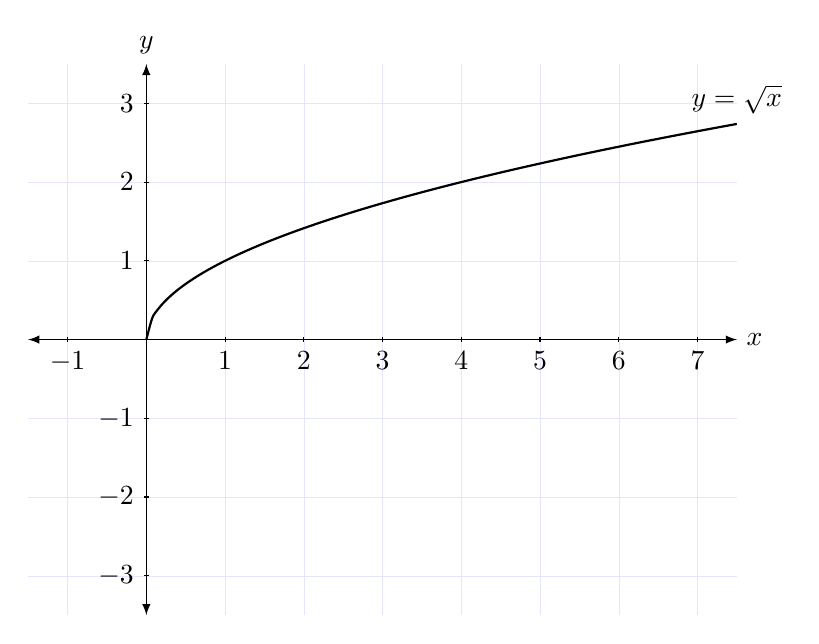
\begin{tikzpicture}[domain=-2:2,samples=100,scale=1.0,>=latex]
\tikzset{bgrid/.style={help lines,color=blue!10,very thin}}

\draw[bgrid] (-1.5,-3.5) grid (7.5,3.5);

\draw[<->, color=black] (-1.5,0) -- (7.5,0) node[right] {$x$};
\draw[<->, color=black] (0,-3.5) -- (0,3.5) node[above] {$y$};

\foreach \x/\xtext in {-1,1,2,3,4,5,6,7}
\draw (\x cm,1pt) -- (\x cm,-1pt) node[anchor=north] {$\xtext$};

\foreach \y/\ytext in {-3,-2,-1,1,2,3}
\draw (1pt,\y cm) -- (-1pt,\y cm) node[anchor=east] {$\ytext$};

\draw[thick,color=black,domain=0:7.5,smooth]
plot (\x,{sqrt(\x)}) node[anchor=south] {$y = \sqrt{x}$};


\end{tikzpicture}
\end{document}